\documentclass[journal]{IEEEtran}
\usepackage[a5paper, margin=10mm]{geometry}
%\usepackage{lmodern} % Ensure lmodern is loaded for pdflatex
\usepackage{tfrupee} % Include tfrupee package

%iffalse
\let\negmedspace\undefined
\let\negthickspace\undefined
\usepackage{gvv-book}
\usepackage{gvv}
\usepackage{cite}
\usepackage{amsmath,amssymb,amsfonts,amsthm}
\usepackage{algorithmic}
\usepackage{graphicx}
\usepackage{textcomp}
\usepackage{xcolor}
\usepackage{txfonts}
\usepackage{listings}
\usepackage{enumitem}
\usepackage{mathtools}
\usepackage{gensymb}
\usepackage{comment}
\usepackage[breaklinks=true]{hyperref}
\usepackage{tkz-euclide} 
\usepackage{listings}                                        
%\def\inputGnumericTable{}                                 
\usepackage[latin1]{inputenc}                                
\usepackage{color}                                            
\usepackage{array}                                            
\usepackage{longtable}                                       
\usepackage{calc}                                             
\usepackage{multirow}                                         
\usepackage{hhline}                                           
\usepackage{ifthen}                                           
\usepackage{lscape}
\usepackage{tabularx}
\usepackage{array}
\usepackage{float}
\usepackage{multicol}

\newcommand{\BEQA}{\begin{eqnarray}}
\newcommand{\EEQA}{\end{eqnarray}}
%\newcommand{\define}{\stackrel{\triangle}{=}}

\setlength{\headheight}{1cm} % Set the height of the header box
\setlength{\headsep}{0mm}     % Set the distance between the header box and the top of the text


%\usepackage[a5paper, top=10mm, bottom=10mm, left=10mm, right=10mm]{geometry}


\setlength{\intextsep}{10pt} % Space between text and floats

% Marks the beginning of the document
\begin{document}
\onecolumn
\bibliographystyle{IEEEtran}
\vspace{3cm}

%\renewcommand{\theequation}{\theenumi}
\numberwithin{equation}{enumi}
\numberwithin{figure}{enumi}
\renewcommand{\thefigure}{\theenumi}
\renewcommand{\thetable}{\theenumi}

\title{Title Undecided}
\author{Shiven Bajpai}
\maketitle

\renewcommand{\thefigure}{\theenumi}
\renewcommand{\thetable}{\theenumi} 

\textbf{Question: } Given that
\begin{align}
	g(t) &= e^{-at}u(t) + e^{bt}u(-t) \label{q1}\\
	u(t) &= \begin{cases}
		0, & t<0\\
		\frac{1}{2}, & t=0 \\
		1, & t>0
	\end{cases} \label{q2}\\
	\int_{-\infty}^{\infty} g(t) &= 1 \label{q3}
\end{align}

Find the possible values of $(a,b)$ if these are the end points of the latus recta of the associated conic. Plot $g(t)$ for these values of $(a,b)$

\bigskip

\textbf{Solution: } We expand the integral as 

\begin{align}
	\int_{-\infty}^{\infty} g(t) &= \int_{-\infty}^{0} g(t) + \int_{0}^{\infty} g(t)\\
	&= \int_{-\infty}^{0} e^{bt} + \int_{0}^{\infty} e^{-at}\\
	&= \frac{1}{b} + \frac{1}{a} \label{integral_result}
\end{align}

Subsituting \eqref{q3} in \eqref{integral_result}

\begin{align}
	\frac{1}{a} + \frac{1}{b} &= 1\\
	ab - a - b &= 0 \label{conic_ab}
\end{align}

Which is the equation of a conic. 
If we take $a$ to be $x$ and $b$ to be $y$ and then express this as a conic in standard form we get

\begin{align}
	\text{g}(\vec{x}) = \vec{x}^\text{T}\vec{Vx} + 2\vec{u}^\text{T}\vec{x} + f \label{actual_conic}
\end{align}

By comparison we obtain:

\begin{align}
	\vec{V} &= \myvec{0 & \frac{1}{2} \\ \frac{1}{2} & 0}\\
	\vec{u} &= \myvec{-\frac{1}{2} \\ -\frac{1}{2}}\\
	f &= 0
\end{align}

We eigen decompose $\vec{V}$ as 

\begin{align}
	\vec{V} &= \vec{PDP}^\text{T}\\
	\vec{P} &= \myvec{\frac{1}{\sqrt{2}} & \frac{1}{\sqrt{2}} \\ \frac{1}{-\sqrt{2}} & \frac{1}{\sqrt{2}}}\\
	\vec{D} &= \myvec{\frac{1}{2} & 0 \\ 0 & \frac{-1}{2}}
\end{align}

And convert the conic into a standard conic to make it simpler to solve using affine transformations.

\begin{align}
	\vec{y}^\text{T}\brak{\frac{\vec{D}}{f_0}}\vec{y} &= 1\\
	\vec{x} &= \vec{Py} + \vec{c} \label{t1}\\
\end{align}

Where 

\begin{align}
	f_0 &= \vec{u}^\text{T}\vec{V}^{-1}\vec{u} - f = 1\\
	\vec{c} &= -\vec{V}^{-1}\vec{u} = \myvec{1 \\ 1}
\end{align}

Since eigenvalues of $\vec{D}$ are $\lambda_1 = \frac{1}{2}$ and $\lambda_2=-\frac{1}{2}$ We use another transformation to shift the negative eigenvalue of $\vec{D}$ to get the hyperbola in standard form, finally giving us

\begin{align}
	\vec{z}^\text{T}\brak{\frac{\vec{D_0}}{f_0}}\vec{z} &= 1\\
	\vec{z}^\text{T}\vec{D_0}\vec{z} - f_0 &= 0  \label{standard_conic}\\
	\vec{y} &= \vec{P}_0\vec{z} \label{t2}\\
\end{align}

Here $\vec{P}_0$ is the reflection matrix $\myvec{0 & 1 \\ 1 & 0}$ and $\vec{D}_0$ is defined as 

\begin{align}
	\vec{D} &= \vec{P}_0\vec{D}_0\vec{P}_0^\text{T}\\
	\vec{P}_0^\text{T}\vec{D}\vec{P}_0 &= \vec{D}_0\\
	\vec{D}_0 &= \myvec{\frac{-1}{2} & 0 \\ 0 & \frac{1}{2}}
\end{align}

Now we solve to find the endpoints of the latus recta of this standard conic

\begin{align}
	\vec{n} &= \sqrt{\lambda_2}\vec{p}_1 = \myvec{\frac{1}{\sqrt{2}} \\ 0}\\
	e &= \sqrt{1 - \frac{\lambda_1}{\lambda_2}} = \sqrt{2}\\
	c &= \dfrac{e\vec{u}^\text{T}\vec{n} \pm \sqrt{e^2 (\vec{u}^T \vec{n})^2 - \lambda_2(e^2 - 1)(\Vert \vec{u} \Vert^2-\lambda_2f)}}{\lambda_2e(e^2 - 1)}\\
	&= \pm \frac{1}{\sqrt{2}}\\
	\vec{F} &= \dfrac{ce^2\vec{n}-\vec{u}}{\lambda_2} = \pm 2 \vec{e}_1\\
\end{align}

Equation of latus recta is

\begin{align}
	\vec{n}^\text{T}\vec{x} &= \vec{n}^\text{T}\vec{F}\\
	\equiv \vec{n}^\text{T}\vec{x} &= 2 \label{latus_rectum} 
\end{align}

Let $\vec{\hat{z}}$ be the endpoints of the latus recta.

From \eqref{latus_rectum} we can say $\vec{\hat{z}}$ is of the form $\myvec{\pm2 \\ k_i}$. Subsituting back in \eqref{standard_conic}

\begin{align}
	\vec{z}^\text{T}\vec{D_0}\vec{z} - f_0 &= 0\\
	-2 + \frac{k_i^2}{2} + 1 &= 0\\
	k_i^2 &= 2\\
	k_i &= \pm \sqrt{2}\\
	\therefore \vec{\hat{z}} &= \myvec{\pm 2 \\ \pm \sqrt{2}}
\end{align}

Now transforming $\vec{\hat{z}}$ back using \eqref{t1}, \eqref{t2} to get endpoints of original conic $\vec{\hat{x}}$.

\begin{align}
	\vec{\hat{x}} &= \vec{P}\brak{\vec{P}_0 \vec{\hat{z}}} + \vec{c}
\end{align}

Which gives us values of $\vec{\hat{x}}$ to be

\begin{align*}
	\vec{\hat{x}}_1 &= \myvec{-\sqrt{2} \\ 2-\sqrt{2}}\\
	\vec{\hat{x}}_2 &= \myvec{\sqrt{2} \\ 2+\sqrt{2}}\\
	\vec{\hat{x}}_3 &= \myvec{2-\sqrt{2} \\ -\sqrt{2}}\\
	\vec{\hat{x}}_4 &= \myvec{2+\sqrt{2} \\ \sqrt{2}}\\
\end{align*}

We can plot out the original conic in \eqref{actual_conic} to verify our solution

\begin{figure}[H]
	\centering
	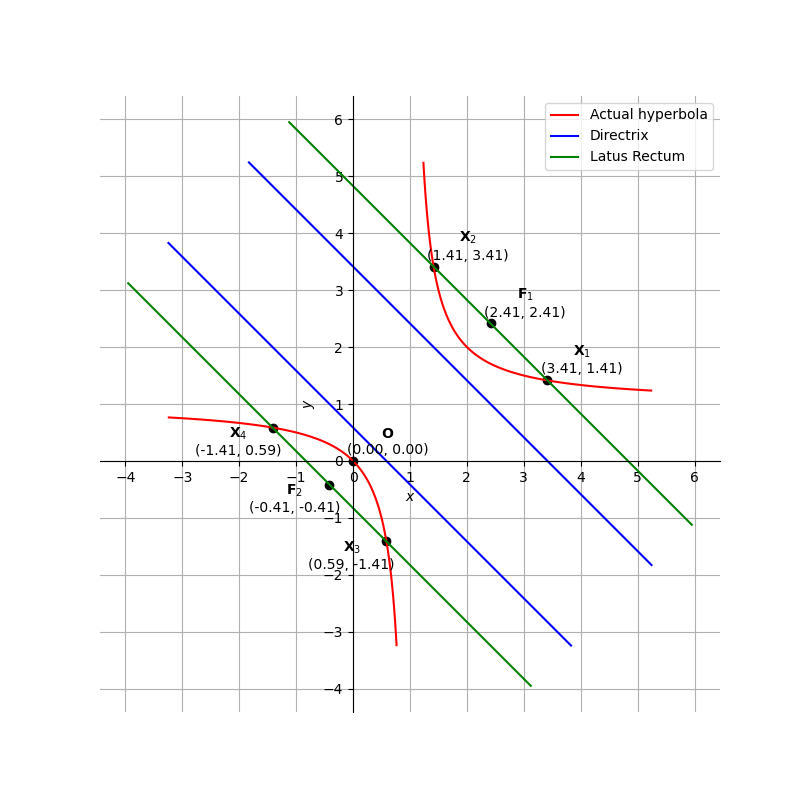
\includegraphics[width=0.75\columnwidth]{Figures/Hyperbola.png} 
	\caption{}
	\label{fig:Hyperbola}
\end{figure}

Out of these, $\vec{\hat{x}}_1$ and $\vec{\hat{x}}_3$ are unfit to be used as values for $(a, b)$ as negative values of $a$ or $b$ will cause $g(t)$ to tend to infinity near $t = 0$ and thus the integral in \eqref{q3} will not converge and condition will not be met.\\

Lastly, We plot the function $g(t)$ for $(a, b) = \vec{\hat{x}}_2$ and $(a, b) = \vec{\hat{x}}_4$

\begin{figure}[H]
	\centering
	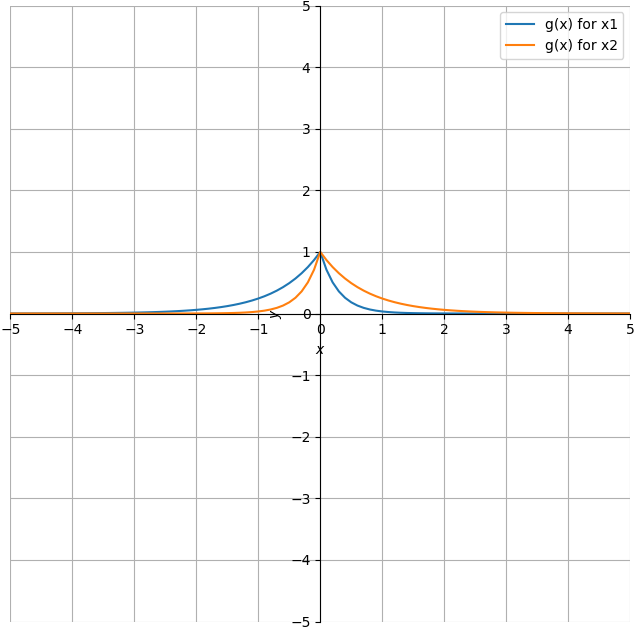
\includegraphics[width=0.75\columnwidth]{Figures/function.png} 
	\caption{}
	\label{fig:Function}
\end{figure}

Code for Figures \ref{fig:Hyperbola} and \ref{fig:Function} can be found at:
\begin{lstlisting}
Codes/hyperbola.py
Codes/function.py
\end{lstlisting}

\end{document}